\chapter{Introduction}
\label{chap:intro}

\todo*{General intro text comes here}

\section{Related work: optimization and stochastic modeling}
\label{sec:intro:relwork}

In the literature there are two main approaches to the optimization of designs according to stochastic metrics and constraints. The first approach solves the optimization problem directly on the level of the stochastic model. In this case, traceability links may be followed to pull back the results of the optimization to the engineering design.

In contrast, higher-level methods perform optimization directly over engineering models are more widespread. However, a downside of the higher-lever approach is that formal models must be constructed from the engineering model to evaluate stochastic metrics, which requires annotating the engineering model or developing a transformation from scratch. Moreover, the lack of deep integration between the transformation and the analysis tool may lead to inefficiencies.

EvoChecker by \citet{Gerasimou15evochecker} was one of the first tools for the optimization on stochastic models using evolutionary techniques, such as the \textabbr{NSGA-II} genetic algorithm~\citep{Deb02nsga}. This approach was extended to support the synthesis of robust design by \citet{Calinescu17robust} in the \textabbr{RODES} synthesis tool~\citep{Calinescu17rodes}.

The testing---as opposed to optimizing---non-functional software requirements by search-based techniques is a related area of research. Literature in the area was surveyed by \citet{Afzal09testing}, as well as \citet{Parasa16testing}, who notes the applicability of EvoChecker to the task.

Search-based techniques are also applied to formal models run time adaptation. \citet{Epifani09adaptation} combined Bayesian estimation and stochastic modeling for run time adaptation in the \textabbr{KAMI} tool. The Activ\mixedabbr{FORMS} runtime environment for architecture-based adaptation employs statistical model checking by simulation to evaluate non-functional requirements~\citep{Iftikhar17activforms}.

Synthesis of optimal policies in Markov decision processes is another common optimization task for stochastic models~\citep{Baier17maximizing}. \citet{Mason17assurance} provided assurance for the correctness of policies learned with reinforcement learning by employing stochastic verification. Abstractions based on Markov decision processes were exploited also by \citet{Quatmann16mdp} for optimizing parameters of stochastic models. 

On the other hand, the number of approaches for deriving stochastic models from engineering models, such as \textabbr{UML}~\citep{Rumbaugh04uml}, Sys\mixedabbr{ML}~\citep{Friedenthal16sysml}, \textabbr{AADL}~\citep{Feiler12aadl} or Palladio~\citep{Becker08palladio} instance models is much larger. Fourteen \textabbr{UML} profiles for dependability analysis were surveyed by \citet{Bernardi08umlprofile}. A more recent survey on the topic is that of \citet{Koziolek10review}.

A general approach for the optimization of engineering models according to stochastic metrics was proposed by \citet{Koziolek11generic}. They provide and encoding for architectural models that enables the application of search-based techniques, such as genetic algorithms, for optimization. The PerOpteryx~\citep{Martens10evolutionary} framework applies this encoding for architectures defined in with Palladio Component Model~\citep{Becker08palladio} for evolutionary optimization. The metrics for optimization can be defined by discrete-event simulations, layered queuing networks~\citep{Franks09lqn} and discrete-time Markov chains~\citep{Koziolek09dependencies}.

We further survey the literature on modular stochastic modeling formalisms and queries in \vref{sec:rgspn:relwork}, while incremental transformation approaches are reviewed in \vref{chap:transform:relwork}.

\section{Overview of our approach}
\label{sec:intro:approach}

In our current work we aim to propose an approach for the construction of stochastic models from engineering models without human intervention in order to evaluate automatically derived architecture proposals in design-space exploration by stochastic analysis.

The proposed transformation process is flexible in the sense that---instead of basing our approach on a single engineering modeling language---the creation of transformations for new architectural domain-specific languages (\textAbbr{DSL}s) in new problem domains are supported without demanding additional specialized knowledge from the users.

\begin{figure}
  \centering
  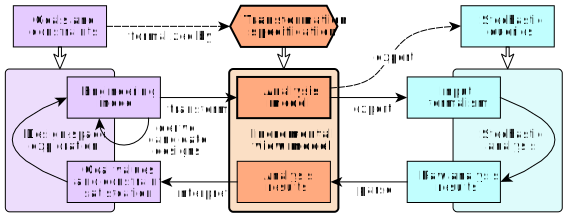
\includegraphics[scale=0.9]{figures/overview}
  \caption{Incremental view transformation as a bridge between design-space exploration and stochastic analysis tools.}
  \label{fig:intro:overview}
\end{figure}

The architecture the proposed solution in the context of design-space exploration and stochastic analysis is shown in \vref{fig:intro:overview}. Components that are highlighted in bold are were developed as part of this work.

Design-space exploration with stochastic metrics is achieved by the interaction of three components. The \emph{design-space explorer} employs (meta-)heuristics to \emph{derive candidate designs} according to the \emph{constraints and goal functions} defined by the user. A candidate design, embodied in some \emph{engineering model} formalism, is analyzed with our toolchain and an external analysis tool, yielding the \emph{values of goal function and information whether the design satisfies the constraints.} Heuristics account for this information when proposing new designs.

The \emph{stochastic analysis} tool is responsible for solving formal stochastic models, such as continuous-time Markov chains~(see \vref{ssec:background:ctmc}). The model to be solved is given in the \emph{input formalism} of the analysis tool. \emph{Stochastic queries,} such as the computations of dependability and performability metrics or the determination whether some probabilistic safety properties are satisfied, are answered to produce \emph{raw analysis results}. 

The \emph{incremental view model transformation}, which is the main focus of our work, bridges the conceptual gap between the engineering formalism employed in \textabbr{DSE} and formal stochastic models in stochastic analysis. The \emph{transformation specification} describes how the formal \emph{analysis model} is constructed from engineering models and formalizes the goals and constraints to be analyzed. The analysis model is \emph{exported} to the input format of the analysis tool. The stochastic queries to be posed are also automatically generated from the analysis model in order to enable dependence on its structure.

The raw analysis results are \emph{parsed} after running the external solver to yield the \emph{analysis results.} The results are interpreted according to the traceability links maintained by the view transformation engine to determine the values of goal functions and constraints.

The requirements for the analysis model formalism were determined to be as follows:
\begin{enumerate*}
\item It should be easy to use for engineers, preferably by building on an existing stochastic modeling formalism.
\item Portability and compatibility with a variety of external analysis tools should be ensured.
\item The analysis model should define not only the stochastic model, but also the posed queries for analysis.
\end{enumerate*}

In turn, the transformation engine that assembles the analysis model should satisfy the following requirements:
\begin{enumerate*}
\item The transformation should be \emph{parametric} in the sense that its behavior is determined by the transformation specification provided by user.
\item The analysis model should be compatible with external analysis tools by avoiding features that are not widely supported in stochastic analysis.
\item End-to-end-traceability should be provided to allow interpretation of analysis results in the context of the engineering model, as well as the analysis model.
\item Incremental execution is preferred, which enables minimizing the work required for updating the analysis model if the engineering model is modified in-place by the \textabbr{DSE} tool. As it will be described in \cref{chap:apply}, in-place modification often occurs in many \textabbr{DSE} paradigms~\citep{Vanherpen14patterns}.
\end{enumerate*}

Our approach differs significantly from existing methods in the literature. In contrast with tools that directly optimize stochastic models~\citepeg{Gerasimou15evochecker,Calinescu17rodes}, we derive an analysis model along with traceability information from engineering models in order to enable design-space exploration with engineering models and stochastic metrics. However, we note that the produced formal models may be transferred to a stochastic model optimizer. The traceability links let user pull back the results of the lower-level optimization to the engineering model; therefore the two approaches can be viewed as complementary.

Compared to transformations for particular modeling languages, such as \textabbr{UML}~\citepeg{Bernardi03building}, our approach is parametric in the transformation specification to allow mappings for any source modeling language. In contrast with the genetic encoding in the PerOpteryx framework~\citep{Koziolek11generic}, our approach does not presume a specific encoding for models and instead transform the engineering models themselves. However, as our work delegates optimization by design-space exploration to a \textabbr{DSE} tool, such encodings may be employed by the selected design-space explorer.

The rest of this work is structures as follows: \Cref{chap:background} recalls some preliminaries in model-based engineering and stochastic analysis. \Cref{chap:rgspn} proposes a formalism for analysis models based on modular Petri nets~\citep{Kindler09modular} in order to ensure user familiarity and portability across analysis tools. \Cref{chap:transform} presents and incremental transformation engine that uses view transformation and graph query preconditions~\citep{Debreceni14viewmodel} to construct the analysis models. \Cref{chap:apply} describes the application of transformation framework in \textabbr{DSE} toolchains and empirically evaluates is scalability. Lastly, we conclude our thesis in \cref{chap:conclusion}.

Two case studies are presented in appendices. The dining philosophers case study in \cref{app:phils} is used throughout the thesis as a running example. A more complex example is shown in \cref{app:architecture}, which transforms architectural models to stochastic Petri nets for hazard rate analysis. The transformations was used in a collaboration with an industrial partner to evaluate safety requirements in a redundant, self-diagnosing automotive system.

%%% Local Variables:
%%% mode: latex
%%% TeX-master: "../main"
%%% End:
